\subsection{Caso de uso 2.1: Confirmar teléfono celular} \label{cu2_1}
\subsubsection{Resumen}
Este caso de uso le permite al usuario confirmar su teléfono celular ingresando el código que fue enviado al número que proporciono al registrarse.
\subsubsection{Descripción}
\begingroup
\setlength{\LTleft}{-10cm plus -1fill}
\setlength{\LTright}{\LTleft}
\begin{center}
  \addtocounter{table}{-1}
    \captionof{table}{Caso de uso 2.1: Confirmar cuenta} \label{tab:cu2_1_tab}
  \begin{longtable}{| p{3.5cm} | p{11.5cm} |}
        \hline
      	\textbf{Versión} &  0.1 \\
        \hline 
       	\textbf{Autor} & Juan Gerardo Diaz Rodarte\\
        \hline
          \textbf{Estatus} & Edición \\
        \hline  
          \textbf{Fecha de último estatus} &  3 de abril de 2017 \\
        \hline
      \multicolumn{2}{|c|}{\large{Atributos}} \\
        \hline
          \textbf{Actor} & Ususario y Sub-Usuario \\
        \hline	
          \textbf{Propósito} &  Permite al usuario confirmar su teléfono celular. \\
        \hline
          \textbf{Disparador} & El actor se registro exitosamente y es redirecionado. \\
        \hline	
          \textbf{Entradas} &
	  \begin{itemize}
	    \item \textbf{Código de confirmación}: Se escribe con el teclado.
	  \end{itemize} \\
        \hline	
          \textbf{Salidas} & 
            \begin{itemize}
              \item \textbf{Interna}: Se mostrará el mensaje MSJ que indica que la cuenta fue confirmada exitosamente.
            \end{itemize} \\
        \hline	
          \textbf{Precondiciones} & 
            \begin{itemize}
              \item \textbf{Interna}: El actor debe haber sido registrado previamente en el sistema.
            \end{itemize} \\
        \hline	
          \textbf{Postcondiciones} & 
            \begin{itemize}
              \item \textbf{Interna}: El teléfono celular del usuario quedara confirmado.
            \end{itemize} \\
        \hline
          \textbf{Reglas de negocio} &
            \begin{itemize}
              \item \textbf{\ref{rnl_01}}
              \item \textbf{\ref{rnrv_09}}
            \end{itemize} \\
        \hline
          \textbf{Mensajes} & 
            \begin{itemize}
              \item \textbf{\ref{msja_01}}
              \item \textbf{\ref{msjc_01}}
              \item \textbf{\ref{msjn_02}}
              \item \textbf{\ref{msjn_03}}
              \item \textbf{\ref{msje_09}}
            \end{itemize} \\
        \hline
          \textbf{Tipo} & Secundaria\\
        \hline	    
  \end{longtable}
\end{center}
\endgroup

\subsubsection{Trayectorias del caso de uso}
\textbf{Trayectoria principal}
\begin{enumerate}
  \item {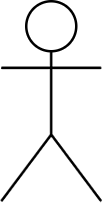
\includegraphics[scale=.1]{Capitulo3/img/actor.png} Termina exitosamente su registro en la vista IU Registrate.}
  \item {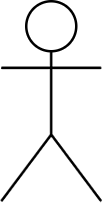
\includegraphics[scale=.1]{Capitulo3/img/actor.png} Ingresa el código que se le fue asignado.}
  \item {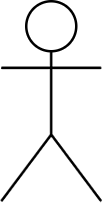
\includegraphics[scale=.1]{Capitulo3/img/actor.png} Presiona el botón para solicitar la confirmación de su cuenta.}
  \item {
\includegraphics[scale=.05]{Capitulo3/img/proceso.png} Verifica que el usuario haya ingresado la información requerida como establecido en la \textbf{\ref{rnl_01}}. \hyperref[cu2_1_ta_a]{[Trayectoria alternativa A]}}
  \item {
\includegraphics[scale=.05]{Capitulo3/img/proceso.png} Verifica que el código ingresado sea válido y corresponda al actor. \hyperref[cu2_1_ta_b]{[Trayectoria alternativa B]}}
  \item {
\includegraphics[scale=.05]{Capitulo3/img/proceso.png} Se muestra el mensaje \textbf{\ref{msjn_03}} que indica la confirmación exitosa del teléfono celular.}
  \item {
\includegraphics[scale=.05]{Capitulo3/img/proceso.png} Se redirecciona a la vista de hogar.}
    \item {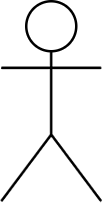
\includegraphics[scale=.1]{Capitulo3/img/actor.png} Hacer uso del sistema.} \\
  \textit{Fin de caso de uso} \\	
\end{enumerate}

\textbf{Trayectoria alternativa A} \phantomsection\label{cu2_1_ta_a} \\
\textbf{Condición:} El actor no proporcionó la información requerida, rompiendo la regla de negocio \textbf{\ref{rnl_01}}.\\
 \begin{enumerate}[label=A\arabic*]
    \item {
\includegraphics[scale=.05]{Capitulo3/img/proceso.png} Muestra el mensaje \textbf{\ref{msja_01}}, indicando que el actor ha dejado campos en blanco.}
    \item {Continua en el paso 5 de la trayectoria principal.} \\
    \textit{Fin de trayectoria} \\
\end{enumerate}

\textbf{Trayectoria alternativa B} \phantomsection\label{cu2_1_ta_b} \\
\textbf{Condición:} El actor ingreso un código invalido, rompiendo la regla de negocio \textbf{\ref{rnrv_09}}. \\
 \begin{enumerate}[label=\arabic*]
    \item {
\includegraphics[scale=.05]{Capitulo3/img/proceso.png} Muestra el mensaje \textbf{\ref{msje_09}}, indicando que el código ingresado no es válido. }
    \item {Continua en el paso 2 de la trayectoria principal.} \\
    \textit{Fin de trayectoria} \\
\end{enumerate}

\textbf{Trayectoria alternativa C} \phantomsection\label{cu2_1_ta_c} \\
\textbf{Condición:} El actor oprime el botón Enviar nuevo código.\\
 \begin{enumerate}[label=\arabic*]
    \item {
\includegraphics[scale=.05]{Capitulo3/img/proceso.png} Se muestra el mensaje de confirmación \textbf{\ref{msjc_01}}.}
    \item {
\includegraphics[scale=.05]{Capitulo3/img/proceso.png} Se envía un nuevo código a la dirección de correo eletrónico del actor.}
    \item {
\includegraphics[scale=.05]{Capitulo3/img/proceso.png} Muestra el mensaje \textbf{\ref{msjn_02}}, indicando que el nuevo código ha sido enviado. }
    \item {Continua en el paso 2 de la trayectoria principal.} \\
    \textit{Fin de trayectoria} \\
\end{enumerate}